\documentclass{beamer}
\usepackage[utf8]{inputenc}
\usepackage{amsthm}
\usepackage{tikz}
\usepackage{circuitikz}
\usetikzlibrary{arrows, positioning}
\usepackage{algorithmic}
\usepackage{tabularx}

\usepackage{amsmath}
\usepackage[utf8]{inputenc}
\usepackage{amsmath}  % For advanced mathematical typesetting
\usepackage[ruled,vlined]{algorithm2e}  % For writing algorithms
\usetikzlibrary{calc}
% \usetikzlibrary{crypto.symbols}
\usetikzlibrary {positioning}
\usetikzlibrary{shapes}

\usetikzlibrary{arrows, positioning}
% Referance
\usepackage[backend=biber]{biblatex}
\addbibresource{main.bib}

\usepackage{listings}
\usepackage{xcolor}
\lstset{
  language=Python,
  basicstyle=\ttfamily\small,
  keywordstyle=\color{blue},
  commentstyle=\color{gray},
  stringstyle=\color{orange},
  numbers=left,
  numberstyle=\tiny\color{gray},
  stepnumber=1,
  numbersep=5pt,
  breaklines=true,
  showstringspaces=false,
  tabsize=4
}
\setbeamertemplate{caption}[numbered]

\usetheme{Madrid}
\usecolortheme{default}

%------------------------------------------------------------
%This block of code defines the information to appear in the
%Title page
\title[MILP IN
CRYPTANALYSIS ] %optional
{USAGE OF MIXED INTEGER
LINEAR PROGRAMMING IN
CRYPTANALYSIS OF BLOCK
CIPHERS}


\author[Halil İbrahim Kaplan] % (optional)
{Halil İbrahim Kaplan }

\institute[] % (optional)
{
  Istanbul Technical University\\
  Informatics Institute
}

\date[2025] % (optional)
{2025}



%End of title page configuration block
%------------------------------------------------------------



%------------------------------------------------------------
%The next block of commands puts the table of contents at the 
%beginning of each section and highlights the current section:

\AtBeginSection[]
{
  \begin{frame}
    \frametitle{Table of Contents}
    \tableofcontents[currentsection]
  \end{frame}
}
%------------------------------------------------------------


\begin{document}

%The next statement creates the title page.
\frame{\titlepage}


%---------------------------------------------------------
%This block of code is for the table of contents after
%the title page
\begin{frame}
\frametitle{Table of Contents}
\tableofcontents
\end{frame}
%---------------------------------------------------------
\section{Preliminaries}

\begin{frame}{Block Ciphers}
    Block ciphers designed to securely
encrypt and decrypt fixed-size blocks of data by transforming plaintext into ciphertext
using a symmetric key. 

\begin{figure}
    \centering
    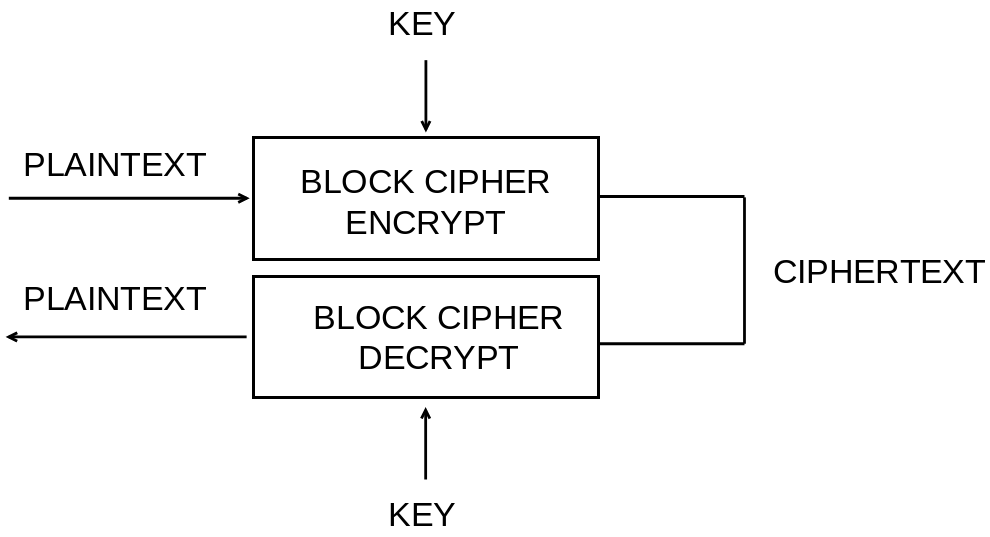
\includegraphics[width=0.5\linewidth]{fig/Screenshot from 2025-08-28 11-23-09.png}
    \caption{Block Cipher Encrytion and Decryption}
    \label{fig:placeholder}
\end{figure}


\end{frame}


\begin{frame}{Cryptanalysis}

    The main
purpose of cryptanalysis:
 \begin{itemize}
    \item Prove that an algorithm is secure against known attacks
in the open literature

    \item Find better complexities for those attacks and contribute to the
security of the algorithm

    \item Break it ! (breaking an algorithm means obtaining the
key with a lower complexity than the algorithm claims.)
    
 \end{itemize}

\end{frame}



\section{MILP}

%---------------------------------------------------------
\begin{frame}{Mixed-Integer Linear Programming (MILP)}
\textbf{Goal:} Optimize (maximize or minimize) a linear function.

\[
 c_1x_1 + c_2x_2 + \dots + c_nx_n
\]

\textbf{Constraints:}
\[
a_{11}x_1 + a_{12}x_2 + \dots + a_{1n}x_n \leq b_1
\]
\[
\vdots
\]
\[
a_{m1}x_1 + \dots + a_{mn}x_n \leq b_m
\]
\[
x_1, x_2, \dots, x_p \in \mathbb{Z}, 
\quad x_{p+1}, \dots, x_n \geq 0
\]

\bigskip
\small
- $x_i$: decision variables \\
- $c_i$: objective function weights \\
- $a_{ij}$: constraint coefficients \\
- $b_j$: limits of constraints
\end{frame}

%---------------------------------------------------------


%---------------------------------------------------------
\begin{frame}{MILP Example}
A company produces two products: \textbf{A} and \textbf{B}.  
The goal: \textbf{maximize profit} under production limits.\\


\[
Z = 40x + 30y
\]

\smallskip
- Profit per unit of A = 40 \\
- Profit per unit of B = 30
\end{frame}

%---------------------------------------------------------
\begin{frame}{MILP Example: Constraints}
\textbf{Constraints:}
\begin{itemize}
    \item \textbf{Labor: } $2x + y \leq 100$ \hfill (100 hours available)
    \item \textbf{Machine: } $x + 3y \leq 90$ \hfill (90 hours available)
    \item \textbf{Demand: } $x \geq 20$ \hfill (min. 20 units of A)
    \item \textbf{Non-negativity: } $x, y \geq 0$
\end{itemize}
\end{frame}

%---------------------------------------------------------
\begin{frame}[fragile]{MILP example}
We will use Sagemath and GLPK solver for modeling.

  

\begin{lstlisting}
p.<x,y> = MixedIntegerLinearProgram(maximization=True, solver="GLPK")
p.set_objective(40*x[0] + 30*y[0])
p.add_constraint(2*x[0] + y[0] == 100)
p.add_constraint(x[0] + 3*y[0] == 90)
p.add_constraint(x[0] >= 20)
p.add_constraint(y[0] >= 0)
print(p.solve())
print(p.get_values(x, y))
\end{lstlisting}

\begin{itemize}
    \item Maximum profit: 2160
    \item A : 42
    \item B : 16
\end{itemize}
    
\end{frame}

\begin{frame}{Cryptanalysis and MILP}

    \begin{figure}
        \centering
        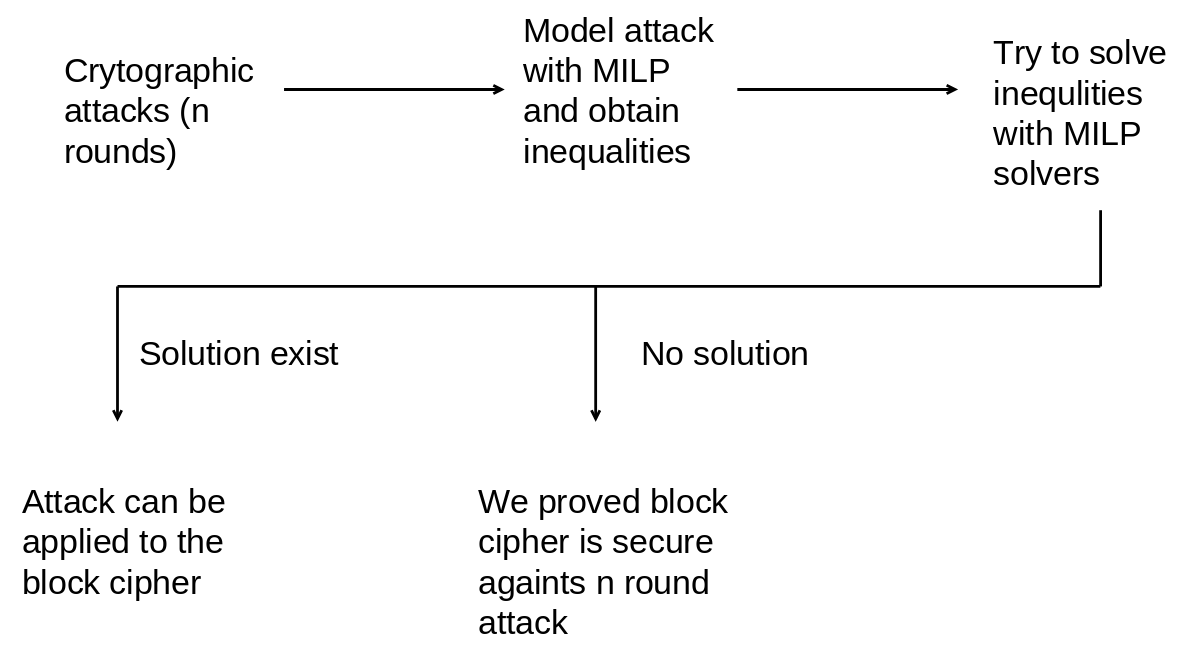
\includegraphics[width=0.75\linewidth]{fig/Screenshot from 2025-08-28 11-42-41.png}
    \end{figure}
    
\end{frame}

%---------------------------------------------------------
\section{Differential Cryptanalysis}


%---------------------------------------------------------
\begin{frame}{Differential Cryptanalysis}
  
\textbf{Idea:}  
Study how input differences between two plaintexts affect output differences in ciphertexts.

\begin{block}{Definition}
For two plaintexts $P$ and $P'$:  
\[
\Delta P = P \oplus P'
\]
\end{block}




\end{frame}


%---------------------------------------------------------
\begin{frame}{Differential Cryptanalysis: Probability}

- Input difference: $\Delta X$ \\ 
- Output difference: $\Delta Y$ \\
\bigskip
\textbf{In an ideal cipher:}  
- For $n$-bit input,  
\[
\Pr[\Delta X \to \Delta Y] = \tfrac{1}{2^n}
\]

\bigskip
\textbf{In practice:}  
- Some input differences lead to output differences with much higher probability.  

\end{frame}

%---------------------------------------------------------

\begin{frame}
\frametitle{Differential Characteristics}

\begin{figure}
    \centering
    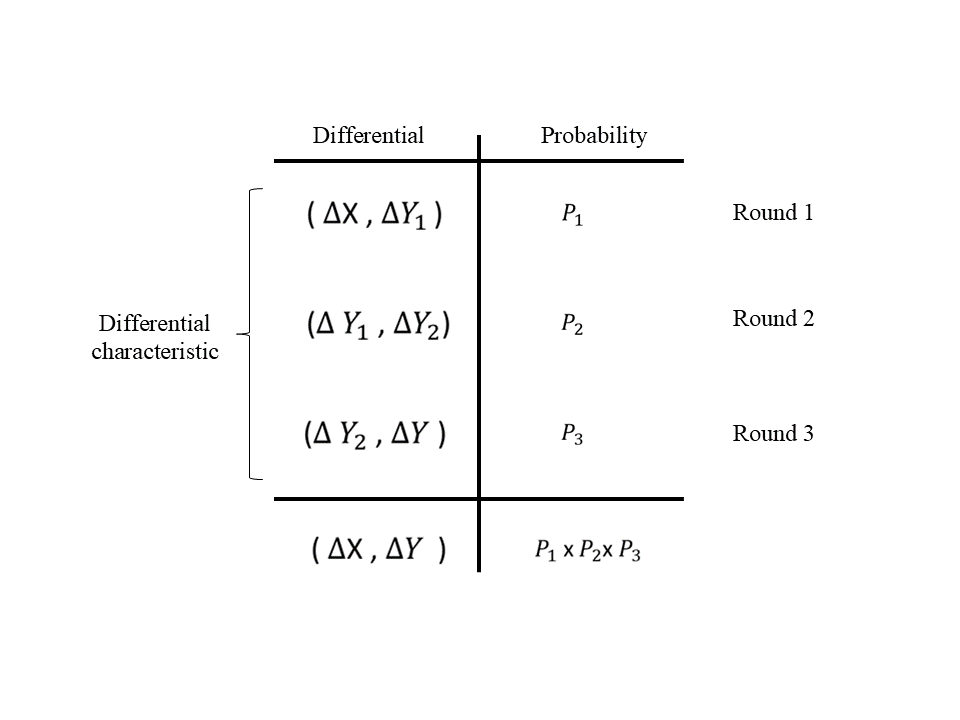
\includegraphics[width=0.8\linewidth]{fig/difchar.png}
    \caption{Concept of constructing differential characteristic}
    \label{fig:difchar}
\end{figure}

\end{frame}


%---------------------------------------------------------
\begin{frame}
\frametitle{Differential Cryptanalysis}


\begin{table}[h!]
\centering
\footnotesize
\begin{tabular}{|c|c|c|c|c|c|c|c|c|c|c|c|c|c|c|c|c|}
\hline
$\Delta X / \Delta Y $ & 0 & 1 & 2 & 3 & 4 & 5 & 6 & 7 & 8 & 9 & A & B & C & D & E & F \\
\hline
0 & 16 & 0 & 0 & 0 & 0 & 0 & 0 & 0 & 0 & 0 & 0 & 0 & 0 & 0 & 0 & 0 \\
\hline
1 & 0 & 0 & 0 & 0 & 0 & 0 & 0 & 0 & 4 & 4 & 4 & 4 & 0 & 0 & 0 & 0 \\
\hline
2 & 0 & 4 & 0 & 4 & 0 & 4 & 4 & 0 & 0 & 0 & 0 & 0 & 0 & 0 & 0 & 0 \\
\hline
3 & 0 & 0 & 0 & 0 & 0 & 0 & 0 & 0 & 2 & 2 & 2 & 2 & 2 & 2 & 2 & 2 \\
\hline
4 & 0 & 0 & 4 & 0 & 0 & 0 & 2 & 2 & 0 & 0 & 0 & 4 & 2 & 2 & 0 & 0 \\
\hline
5 & 0 & 0 & 4 & 0 & 0 & 0 & 2 & 2 & 0 & 0 & 4 & 0 & 2 & 2 & 0 & 0 \\
\hline
6 & 0 & 2 & 0 & 2 & 2 & 0 & 0 & 2 & 2 & 0 & 2 & 0 & 0 & 2 & 2 & 0 \\
\hline
7 & 0 & 2 & 0 & 2 & 2 & 0 & 0 & 2 & 0 & 2 & 0 & 2 & 2 & 0 & 0 & 2 \\
\hline
8 & 0 & 0 & 0 & 0 & 4 & 4 & 0 & 0 & 0 & 0 & 0 & 0 & 2 & 2 & 2 & 2 \\
\hline
9 & 0 & 0 & 0 & 0 & 4 & 4 & 0 & 0 & 0 & 0 & 0 & 0 & 2 & 2 & 2 & 2 \\
\hline
A & 0 & 0 & 0 & 0 & 0 & 4 & 4 & 0 & 2 & 2 & 2 & 2 & 0 & 0 & 0 & 0 \\
\hline
B & 0 & 4 & 0 & 4 & 0 & 0 & 0 & 0 & 0 & 0 & 0 & 0 & 2 & 2 & 2 & 2 \\
\hline
C & 0 & 0 & 4 & 0 & 0 & 0 & 2 & 2 & 4 & 0 & 0 & 0 & 0 & 0 & 2 & 2 \\
\hline
D & 0 & 0 & 4 & 0 & 0 & 0 & 2 & 2 & 0 & 4 & 0 & 0 & 0 & 0 & 2 & 2 \\
\hline
E & 0 & 2 & 0 & 2 & 2 & 0 & 0 & 2 & 0 & 2 & 0 & 2 & 0 & 2 & 2 & 0 \\
\hline
F & 0 & 2 & 0 & 2 & 2 & 0 & 0 & 2 & 2 & 0 & 2 & 0 & 2 & 0 & 0 & 2 \\
\hline
\end{tabular}
\caption{Differential Distribution Table (DDT) of PRINCE algorithm}
\label{tbl:ddtprince}
\end{table} 
    
\end{frame}
%---------------------------------------------------------
\begin{frame}{Steps of Differential Cryptanalysis}
\begin{enumerate}
    \item \textbf{Select Differentials:}  
          Use DDT to find $(\Delta X, \Delta Y)$ pairs with high probability.  
    \item \textbf{Collect Pairs:}  
          Generate many plaintext pairs $P, P'$ with $P \oplus P' = \Delta X$.  
    \item \textbf{Encrypt:}  
          Process these pairs through the cipher.  
    \item \textbf{Analyze Outputs:}  
          Check if observed ciphertext differences match expected $\Delta Y$.  
    \item \textbf{Key Recovery:}  
          Use biases to guess round subkeys (esp. in the last rounds).  
\end{enumerate}
\end{frame}

\begin{frame}{Differential Cryptanalysis}
    

    \begin{figure}
        \centering
        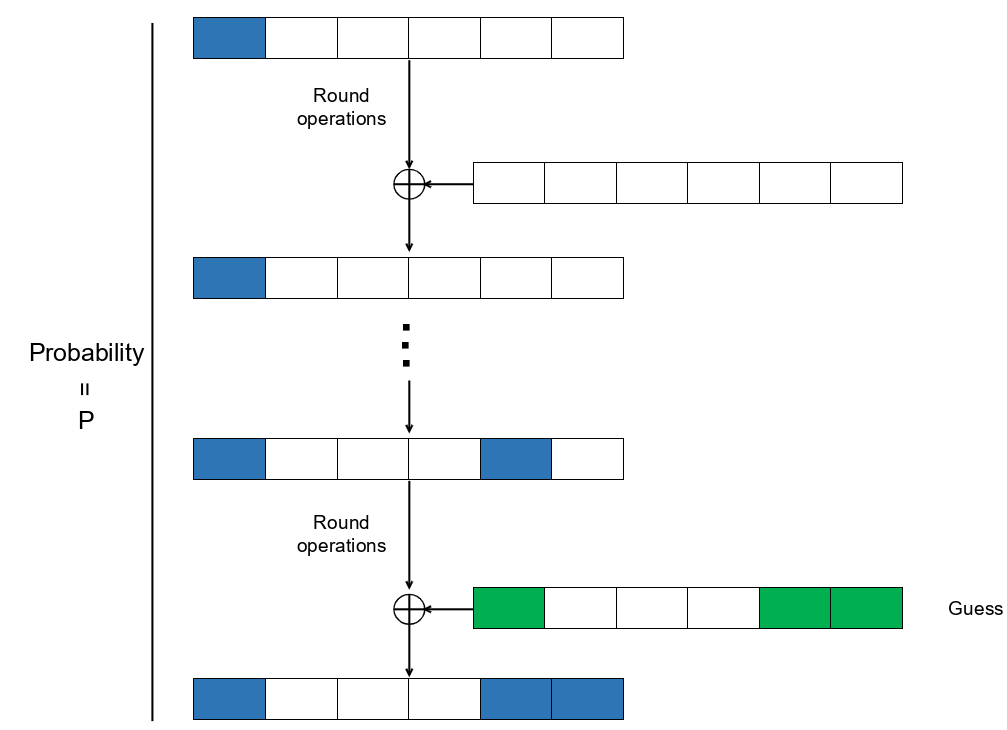
\includegraphics[width=0.7\linewidth]{image.png}
        \caption{Differential Cryptanalysis}
        \label{fig:placeholder}
    \end{figure}
    
\end{frame}

\begin{frame}{Related-key Differential Cryptanalysis}

    Adds differentials also to key sechedule.  

    \begin{figure}
        \centering
        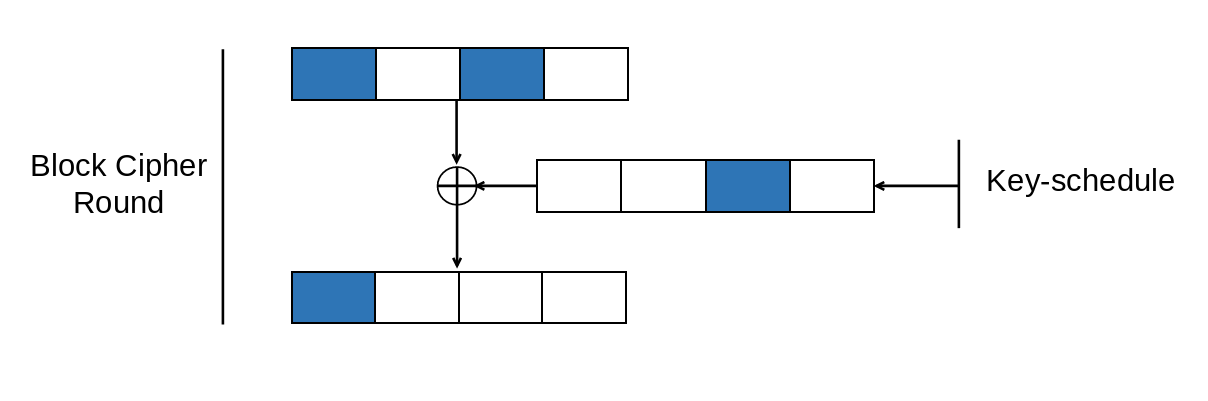
\includegraphics[width=0.7\linewidth]{fig/image.png}
        \caption{Related-key Differential Cryptanalysis}
        \label{fig:placeholder}
    \end{figure}
    
\end{frame}


%---------------------------------------------------------

\section{ITUbee Block Cipher}

%---------------------------------------------------------
\begin{frame}
\frametitle{ITUbee Block Cipher}
\begin{figure}[!ht]
\centering
\resizebox{1\textwidth}{!}{%
\begin{circuitikz}
\tikzstyle{every node}=[font=\Large]

\node [font=\Large] at (2.5,16) {PL};
\draw (2.5,15.5) to[short] (2.5,14.5);
\draw  (2.5,14) circle (0.5cm);
\draw [short] (2.5,13.5) -- (2.5,11.5);
\draw [->, >=Stealth] (2.5,11.5) -- (4,11.5);
\draw  (4,12) rectangle  node {\large F} (5.25,11);
\draw [->, >=Stealth] (5.25,11.5) -- (6.5,11.5);
\draw [short] (2.5,14.5) -- (2.5,13.5);
\draw [short] (2,14) -- (3,14);
\draw  (7,11.5) circle (0.5cm);
\draw [->, >=Stealth] (7.5,11.5) -- (8.75,11.5);
\draw  (11.25,12) rectangle  node {\Large L} (12.5,11);
\draw [->, >=Stealth] (12.5,11.5) -- (14,11.5);
\draw  (14,12) rectangle  node {\Large F} (15.25,11);
\draw [->, >=Stealth] (15.25,11.5) -- (17,11.5);
\draw  (17.5,11.5) circle (0.5cm);
\node [font=\Large] at (17.5,16) {PR};
\draw (17.5,15.5) to[short] (17.5,14.5);
\draw  (17.5,14) circle (0.5cm);
\node [font=\LARGE] at (3,11.75) {};
\draw [short] (17.5,13.5) -- (17.5,12);
\draw [short] (6.5,11.5) -- (7.5,11.5);
\draw [short] (7,12) -- (7,11);
\draw [short] (17,11.5) -- (18,11.5);
\draw [short] (17.5,12) -- (17.5,11);
\draw [short] (17,14) -- (18,14);
\draw [short] (17.5,14.5) -- (17.5,13.5);
\draw [short] (17.5,11) -- (17.5,10.25);
\draw [short] (2.5,11.5) -- (2.5,10.25);
\draw [short] (2.5,10.25) -- (17.5,8.25);
\draw [short] (17.5,10.25) -- (2.5,8.25);
\node [font=\large] at (1.5,14) {KL};
\node [font=\large] at (18.5,14) {KR};
\node [font=\large] at (7,12.5) {KR};
\draw  (9.25,11.5) circle (0.5cm);
\draw [->, >=Stealth] (9.75,11.5) -- (11.25,11.5);
\draw [short] (8.75,11.5) -- (9.75,11.5);
\draw [short] (9.25,12) -- (9.25,11);
\node [font=\Large] at (9.25,12.5) {Rc};
\draw [short] (2.5,8.25) -- (2.5,7.5);
\node [font=\Large] at (3,7.25) {};
\node [font=\Large] at (3,7.25) {};
\node [font=\Large] at (3,7.25) {};
\node [font=\Large] at (3,7.25) {};
\draw [short] (17.5,8.25) -- (17.5,7);
\draw [short] (2.5,8.25) -- (2.5,7);
\end{circuitikz}
}%
\caption{ITUbee round structure}
\label{fig:itubee}
\end{figure}

\end{frame}
%---------------------------------------------------------


%---------------------------------------------------------
\begin{frame}{ITUbee Block Cipher}

\textbf{L Function} 

\[
L(a,b,c,d,e) = (e\oplus a\oplus b,\; a\oplus b\oplus c,\; b\oplus c\oplus d,\; c\oplus d\oplus e,\; d\oplus e\oplus a)
\]
\textbf{F function} \linebreak
    
    \begin{center}
        $F (X) = S(L(S(X)))$
    \end{center}

    \begin{center}
        $S(a\parallel b \parallel c \parallel d \parallel e) = s[a] \parallel s[b] \parallel s[c] \parallel s[d] \parallel s[e]$ 
    \end{center}

\end{frame}

%---------------------------------------------------------
\begin{frame}{ITUbee Block Cipher}

    \textbf{Key Schedule} \linebreak
    
    \begin{itemize}
    \item 80-bit key is split into two 40-bit halves:
    \[
    K = K_L \parallel K_R
    \]
    \item Odd rounds use $K_R$
    \item Even rounds use $K_L$
    \item No dedicated key schedule
\end{itemize}

\end{frame}



%---------------------------------------------------------
\section{MILP representation of block ciphers}

%---------------------------------------------------------

\begin{frame}
\frametitle{MILP Modelling of XOR Operation}

Following \cite{mouha2012differential}, \\
$x_{in1}$, $x_{in2}$ : input differences of XOR \\
$x_{out}$ : output difference of XOR.\\  
The branch number is $2$.

We introduce a binary variable $d$:
\begin{itemize}
    \item $d = 0$ if $x_{in1} = x_{in2} = x_{out} = 0$
    \item $d = 1$ otherwise
\end{itemize}

The XOR is modelled with:


\[
\begin{aligned}
x_{in1} + x_{in2} + x_{out} &\geq 2d \\
d &\geq x_{in1} \\
d &\geq x_{in2} \\
d &\geq x_{out}
\end{aligned}
\]



\end{frame}

\begin{frame}
\frametitle{MILP Modelling of Linear Transformation}

Similarly, for a linear transformation with:
\begin{itemize}
    \item Inputs: $x_{in1}, x_{in2}, \dots, x_{inM}$
    \item Outputs: $x_{out1}, x_{out2}, \dots, x_{outM}$
\end{itemize}

Let $B$ be the branch number and $d$ the dummy variable (as in XOR modelling).

The model is:


\[
x_{in1} + \dots + x_{inM} + x_{out1} + \dots + x_{outM} \geq B \cdot d
\]


and  


\[
d \geq x_{in_{i}},\quad d \geq x_{out_{j}} \quad \forall i,j
\]



\end{frame}

\begin{frame}
\frametitle{MILP Representation of S-boxes}

Goal: minimize the number of \textbf{active S-boxes} to find the best differential trails.

\textbf{Key idea:}
\begin{itemize}
    \item Active input ($\neq 0$) $\Rightarrow$ active output
    \item Passive input ($= 0$) $\Rightarrow$ passive output
\end{itemize}

We only track \textbf{activity} with a binary variable — no internal structure is modelled.
\end{frame}



\begin{frame}
    \frametitle{H-representation example}

    \begin{center}
    $L(a,b,c)=(a \oplus b , a \oplus c , b \oplus c ) \text{ where a,b.c are 2 bit values}  $
\end{center}
\begin{table}[h]
\footnotesize
\centering
\begin{tabular}{|c|c|}
\hline
\textbf{Input Differences} & \textbf{Output Differences} \\ \hline
0 0 0 & 0 0 0 \\ \hline
0 0 1 & 0 1 1 \\ \hline
0 1 0 & 1 0 1 \\ \hline
0 1 1 & 1 1 0 \\ \hline
0 1 1 & 1 1 1 \\ \hline
1 0 0 & 1 1 0 \\ \hline
1 0 1 & 1 0 1 \\ \hline
1 0 1 & 1 1 1 \\ \hline
1 1 0 & 0 1 1 \\ \hline
... & ... \\ \hline
1 1 1 & 1 0 1 \\ \hline
1 1 1 & 1 1 0 \\ \hline
1 1 1 & 1 1 1 \\ \hline
\end{tabular}
\caption{Input and Output Differences of $L$ function}
\label{tab:hreptab}
\end{table}
    
\end{frame}

\begin{frame}
    \frametitle{H-representation example}
\begin{table}[h]
\footnotesize
\centering
\begin{tabular}{|c|l|}
\hline
\textbf{No.} & \textbf{Inequality} \\ \hline
1  & $(0, 0, -1, 0, 0, 0) x + 1 \geq 0$ \\ \hline
2  & $(0, -1, 0, 0, 0, 0) x + 1 \geq 0$ \\ \hline
3  & $(-1, 0, 0, 0, 0, 0) x + 1 \geq 0$ \\ \hline
4  & $(0, 0, 0, -1, 0, 0) x + 1 \geq 0$ \\ \hline
5  & $(0, 0, 0, 0, -1, 0) x + 1 \geq 0$ \\ \hline
6  & $(0, 0, 0, 0, 0, -1) x + 1 \geq 0$ \\ \hline
7  & $(0, -1, 1, 0, 0, 1) x + 0 \geq 0$ \\ \hline
8  & $(0, 0, 0, -1, 1, 1) x + 0 \geq 0$ \\ \hline
... & ... \\ \hline
18 & $(-1, 1, 0, 1, 0, 0) x + 0 \geq 0$ \\ \hline
19 & $(1, -1, -1, 1, 1, -1) x + 1 \geq 0$ \\ \hline
20 & $(1, -1, 0, 1, 0, 0) x + 0 \geq 0$ \\ \hline
21 & $(-1, 1, -1, 1, -1, 1) x + 1 \geq 0$ \\ \hline
22 & $(-1, -1, 1, -1, 1, 1) x + 1 \geq 0$ \\ \hline
\end{tabular}
\caption{H-representation of $L$ function}
\label{tab:h-repineq}
\end{table}
    
\end{frame}

\begin{frame}
\footnotesize
\frametitle{Differential cryptanalysis model with MILP}
\begin{figure}[!ht]
\centering
\resizebox{1\textwidth}{!}{%
\begin{circuitikz}
\tikzstyle{every node}=[font=\large]
\node [font=\large] at (2.5,16) {R1};
\draw (2.5,15.5) to[short] (2.5,14.5);
\draw  (2.5,14) circle (0.5cm);
\draw [short] (2.5,13.5) -- (2.5,11.5);
\draw [->, >=Stealth] (2.5,11.5) -- (4,11.5);
\draw  (4,12) rectangle  node {\large SLS} (5.25,11);
\draw [->, >=Stealth] (5.25,11.5) -- (6.5,11.5);
\draw [short] (2.5,14.5) -- (2.5,13.5);
\draw [short] (2,14) -- (3,14);
\draw  (7,11.5) circle (0.5cm);
\draw [->, >=Stealth] (7.5,11.5) -- (8.75,11.5);
\draw  (8.75,12) rectangle  node {\large L} (10,11);
\draw [->, >=Stealth] (10,11.5) -- (11.5,11.5);
\draw  (11.5,12) rectangle  node {\large SLS} (12.75,11);
\draw [->, >=Stealth] (12.75,11.5) -- (14.5,11.5);
\draw  (15,11.5) circle (0.5cm);
\node [font=\large] at (15,16) {R0};
\draw (15,15.5) to[short] (15,14.5);
\draw  (15,14) circle (0.5cm);
\node [font=\large] at (3,11.75) {};
\draw [short] (15,13.5) -- (15,12);
\draw [short] (6.5,11.5) -- (7.5,11.5);
\draw [short] (7,12) -- (7,11);
\draw [short] (14.5,11.5) -- (15.5,11.5);
\draw [short] (15,12) -- (15,11);
\draw [short] (14.5,14) -- (15.5,14);
\draw [short] (15,14.5) -- (15,13.5);
\draw [short] (15,11) -- (15,10.25);
\draw [short] (2.5,11.5) -- (2.5,10.25);
\draw [short] (2.5,10.25) -- (15,8.25);
\draw [short] (15,10.25) -- (2.5,8.25);
\node [font=\large] at (1.5,14) {KL};
\node [font=\large] at (16,14) {KR};
\node [font=\large] at (7,12.5) {KR};
\node [font=\large] at (3.25,12) {R1};
\node [font=\large] at (5.75,12) {R1a};
\node [font=\large] at (8,12) {R1a};
\node [font=\large] at (10.75,12) {R1b};
\node [font=\large] at (13.75,12) {R1c};
\node [font=\large] at (15.5,10.5) {R2};
\node [font=\large] at (2.5,8) {R2};
\node [font=\large] at (15,8) {R1};
\end{circuitikz}
}%
\caption{ITUbee  MILP differential cryptanalysis sketch}
\label{fig: ITUbeeDif}
\end{figure}

\end{frame}

\begin{frame}
\frametitle{Differential cryptanalysis model with MILP}
\begin{itemize}
    \item Number of Constrains:  18169
    \item Number of Variables:  85
    \item Minimum number of active s-box for 3 round:  16.0
    \item Best probability for s-box: $2^{-6}$
    \item Best probability for 3 round differential characteristic will 
    be $(2^{-6})^{16}= 2^{-96} $
\end{itemize}

which is not usable for differential attack.

\end{frame}


\begin{frame}
\frametitle{Differential cryptanalysis model with MILP}
\begin{table}[H]
    \footnotesize
    \centering
    \begin{tabular}{|c|c|c|}
        \hline
        \textbf{Stage} & \textbf{Binary Index} & \textbf{Characteristic} \\
        \hline
        1. round  & R1 & \{0: 0.0, 1: 0.0, 2: 0.0, 3: 0.0, 4: 1.0\} \\
        input      & R0 & \{0: 0.0, 1: 0.0, 2: 0.0, 3: 0.0, 4: 0.0\} \\
        \hline
        1. round  & R1a & \{0: 1.0, 1: 0.0, 2: 0.0, 3: 1.0, 4: 1.0\} \\
        middle values   & R1b & \{0: 0.0, 1: 1.0, 2: 1.0, 3: 0.0, 4: 1.0\} \\
                   & R1c & \{0: 0.0, 1: 0.0, 2: 0.0, 3: 0.0, 4: 1.0\} \\
        \hline
        2. round& R2 & \{0: 0.0, 1: 0.0, 2: 0.0, 3: 0.0, 4: 1.0\} \\
        input      & R1 & \{0: 0.0, 1: 0.0, 2: 0.0, 3: 0.0, 4: 1.0\} \\
        \hline
        2. round & R2a & \{0: 1.0, 1: 0.0, 2: 0.0, 3: 1.0, 4: 1.0\} \\
        middle values  & R2b & \{0: 0.0, 1: 1.0, 2: 1.0, 3: 0.0, 4: 1.0\} \\
                   & R2c & \{0: 0.0, 1: 0.0, 2: 0.0, 3: 0.0, 4: 1.0\} \\
        \hline
        3. round  & R3 & \{0: 0.0, 1: 0.0, 2: 0.0, 3: 0.0, 4: 0.0\} \\
        input     & R2 & \{0: 0.0, 1: 0.0, 2: 0.0, 3: 0.0, 4: 1.0\} \\
        \hline
        3. round  & R3a & \{0: 0.0, 1: 0.0, 2: 0.0, 3: 0.0, 4: 0.0\} \\
        middle values   & R3b & \{0: 0.0, 1: 0.0, 2: 0.0, 3: 0.0, 4: 0.0\} \\
                   & R3c & \{0: 0.0, 1: 0.0, 2: 0.0, 3: 0.0, 4: 0.0\} \\
        \hline
        4. round & R4 & \{0: 0.0, 1: 0.0, 2: 0.0, 3: 0.0, 4: 1.0\} \\
        input    & R3 & \{0: 0.0, 1: 0.0, 2: 0.0, 3: 0.0, 4: 0.0\} \\
        \hline
    \end{tabular}
    \caption{Best 3 round differential characteristic of ITUbee algorithm}
    \label{tab:MILPcharDif}
\end{table}

\end{frame}

\begin{frame}
\begin{figure}[!ht]
\centering
\resizebox{1\textwidth}{!}{%
\begin{circuitikz}
\tikzstyle{every node}=[font=\large]

\node [font=\large] at (2.5,16) {R1};
\draw (2.5,15.5) to[short] (2.5,14.5);
\draw  (2.5,14) circle (0.5cm);
\draw [short] (2.5,13.5) -- (2.5,11.5);
\draw [->, >=Stealth] (2.5,11.5) -- (4,11.5);
\draw  (4,12) rectangle  node {\large SLS} (5.25,11);
\draw [->, >=Stealth] (5.25,11.5) -- (6.5,11.5);
\draw [short] (2.5,14.5) -- (2.5,13.5);
\draw [short] (2,14) -- (3,14);
\draw  (7,11.5) circle (0.5cm);
\draw [->, >=Stealth] (7.5,11.5) -- (8.75,11.5);
\draw  (8.75,12) rectangle  node {\large L} (10,11);
\draw [->, >=Stealth] (10,11.5) -- (11.5,11.5);
\draw  (11.5,12) rectangle  node {\large SLS} (12.75,11);
\draw [->, >=Stealth] (12.75,11.5) -- (14.5,11.5);
\draw  (15,11.5) circle (0.5cm);
\node [font=\large] at (15,16) {R0};
\draw (15,15.5) to[short] (15,14.5);
\draw  (15,14) circle (0.5cm);
\node [font=\large] at (3,11.75) {};
\draw [short] (15,13.5) -- (15,12);
\draw [short] (6.5,11.5) -- (7.5,11.5);
\draw [short] (7,12) -- (7,11);
\draw [short] (14.5,11.5) -- (15.5,11.5);
\draw [short] (15,12) -- (15,11);
\draw [short] (14.5,14) -- (15.5,14);
\draw [short] (15,14.5) -- (15,13.5);
\draw [short] (15,11) -- (15,10.25);
\draw [short] (2.5,11.5) -- (2.5,10.25);
\draw [short] (2.5,10.25) -- (15,8.25);
\draw [short] (15,10.25) -- (2.5,8.25);
\node [font=\large] at (1.5,14) {KL};
\node [font=\large] at (16,14) {KR};
\node [font=\large] at (7,12.5) {KR};
\node [font=\large] at (3.25,12) {R3};
\node [font=\large] at (5.75,12) {R3a};
\node [font=\large] at (8,12) {R3b};
\node [font=\large] at (10.75,12) {R3c};
\node [font=\large] at (13.75,12) {R3d};
\node [font=\large] at (15.5,10.5) {R4};
\node [font=\large] at (2.5,8) {R4};
\node [font=\large] at (15,8) {R3};
\node [font=\large] at (2,12.5) {R3};
\node [font=\large] at (15.5,12.5) {R2};
\end{circuitikz}
}%
\caption{ITUbee MILP Related-Key Differential Cryptanalysis Sketch}
\label{fig:itubeeRelated}
\end{figure}
\end{frame}

\begin{frame}
\frametitle{Differential cryptanalysis model with MILP}
\begin{itemize}
    \item Number of Constrains:  48649
    \item Number of Variables:  320
    \item Minimum number of active s-box for 8 round:  16.0
    \item Best probability for s-box: $2^{-6}$
    \item Best probability for 8 round differential characteristic will 
    be $(2^{-6})^{16}= 2^{-96} $
\end{itemize}

which is not usable for related-key differential attack.

\end{frame}


\begin{frame}

\begin{table}[ht]
    \footnotesize
    \centering
    \begin{tabular}{|c|c|c|}
        \hline
        \textbf{Stage} & \textbf{Binary Index} & \textbf{Characteristic} \\
        \hline
        Key  & KL & \{0: 0.0, 1: 1.0, 2: 0.0, 3: 1.0, 4: 0.0\} \\
                     & KR & \{0: 0.0, 1: 0.0, 2: 0.0, 3: 0.0, 4: 0.0\} \\
        \hline
        1. round  & R1 & \{0: 0.0, 1: 1.0, 2: 0.0, 3: 1.0, 4: 0.0\} \\
        input     & R0 & \{0: 1.0, 1: 0.0, 2: 0.0, 3: 0.0, 4: 1.0\} \\
        \hline
        1. round  & R2 & \{0: 1.0, 1: 0.0, 2: 0.0, 3: 0.0, 4: 1.0\} \\
        middle values & R3-3a-3b-3c-3d & \{0: 0.0, 1: 0.0, 2: 0.0, 3: 0.0, 4: 0.0\} \\     
        \hline
        2. round  & R4 & \{0: 1.0, 1: 0.0, 2: 0.0, 3: 0.0, 4: 1.0\} \\
        input     & R3 & \{0: 0.0, 1: 0.0, 2: 0.0, 3: 0.0, 4: 0.0\} \\
        \hline
        2. round  & R4a & \{0: 0.0, 1: 1.0, 2: 0.0, 3: 1.0, 4: 0.0\} \\
        middle values & R4b-4c-4d & \{0: 0.0, 1: 0.0, 2: 0.0, 3: 0.0, 4: 0.0\} \\
                      
        \hline
        ...  & ... & ... \\
        
                     
        \hline
        7. round  & R9 & \{0: 0.0, 1: 0.0, 2: 0.0, 3: 0.0, 4: 0.0\} \\
        input     & R8 & \{0: 1.0, 1: 0.0, 2: 0.0, 3: 0.0, 4: 1.0\} \\
        \hline
        7. round middle values & R9a-9b-9c-9d & \{0: 0.0, 1: 0.0, 2: 0.0, 3: 0.0, 4: 0.0\} \\
        \hline
        8. round  & R10 & \{0: 1.0, 1: 0.0, 2: 0.0, 3: 0.0, 4: 1.0\} \\
        input      & R9  & \{0: 0.0, 1: 0.0, 2: 0.0, 3: 0.0, 4: 0.0\} \\
        \hline
        8. round  & R10a & \{0: 0.0, 1: 1.0, 2: 0.0, 3: 1.0, 4: 0.0\} \\
        middle values & R10b-10c-10d & \{0: 0.0, 1: 0.0, 2: 0.0, 3: 0.0, 4: 0.0\} \\
                      
        \hline
        9. round & R11 & \{0: 0.0, 1: 0.0, 2: 0.0, 3: 0.0, 4: 0.0\} \\
        input     & R10 & \{0: 1.0, 1: 0.0, 2: 0.0, 3: 0.0, 4: 1.0\} \\
        \hline
    \end{tabular}
    \caption{Best 8 round related-key differential characteristic of ITUbee algorithm}
    \label{tab:RelatedKeyDif}
\end{table}

\end{frame}

\begin{frame}{Our contribution}


\begin{table}[ht]
    \footnotesize
    \centering
    \begin{tabular}{|c|c|c|c|}
        \hline
        \textbf{Stage} & \textbf{Differential} & \textbf{Linear}  & \textbf{Related-key Differential}  \\
        \hline
        \cite{karakocc2013itubee}  & 3 round & 3 round & 10 round \\
        \hline
        Our Result & 3 round & 3 round & \textbf{8 round }  \\  
        \hline
    \end{tabular}
    \caption{Result Comparison}
    \label{tab:RelatedKeyDif}
\end{table}


\end{frame}

\section{References}

%---------------------------------------------------------
\begin{frame}
\frametitle{References}

\printbibliography

\end{frame}
%---------------------------------------------------------



\end{document}